\section{Technical background}
% \subsection{Related technologies}
% In this section we will briefly analyze and explain related technologies based on the problem statement from section \ref{introduction-background}. We will compare key properties of these technologies and based on the analysis and the process of elimination we will define the relevant technologies for this research.

\label{tech-oview}
% most recent stage in the development of a product, incorporating the newest ideas and features
% add discussion about these tech in introduction or conclusion of this section
% Analyze the requirement for your research questions

In this section we provide an overview of the technologies used in our methodology in sections \ref{pid-poc} and \ref{planning-ndn}. We will briefly analyze and explain related technologies based on the general problem statement in research clouds from section \ref{introduction-background}. We will compare key properties of these technologies and based on the analysis and the process of elimination we will define the relevant technologies for this research.

\label{pid-intr}
Shortly after the introduction of the WWW, Tim Berners Lee (its creator) proposed to the IETF to use the \gls{uri} as the naming schema for identifying contents on the web. This proposal got rejected by the IETF, due to the fact that it does not allow users of the web to change the \gls{uri} of the web contents when moving the web contents to another location. This lead to the use of URLs (Uniform Resource Locators) as the naming schema to identify web content \cite{icn-bd}. 
%In this paper, the term Web content refers to a digital object.
 
The use of URLs did not seem to create issues in the early stages of the web. However, several studies have found out that approximately 50\% of the URLs  in scholarly publications fail to retrieve the digital object after a period of seven to ten years. Web users began to experience the problem of a broken link, or the so called "link rot" problem \cite{rot-link1, rot-link2}. This is a situation where a user fails to retrieve the web content by its URL, due to the fact that the location of the web content has been changed \cite{icn-bd, ark-id}. 

Therefore, the first \gls{pid} systems emerged in the mid-1990s shortly after the introduction of the web itself. A \gls{pid} is a long-lasting, permanent reference to digital objects. Traditional identifiers, such as the bibliographic \gls{isbn} will not be interpreted as a hyperlink by web browsers. For example the string \texttt{ISBN 951-45-9942-X} has to be expressed as a HTTP \gls{uri} in the form of \texttt{\url{http://urn.fi/URN:ISBN:951-45-9942-X}} to be a persistent link to the resource. As shown in the persistent link, the term \gls{urn} is used, which is an example of a \gls{pid} type that is used for object identification. 
PIDs such as \gls{urn} are names which do not imply a location. A \gls{url} identifies the location of a resource identified by a URN. The resource may reside in one or more locations, may move or might not be available at all. A \gls{pid} needs to be mapped to a URL, which is the role of resolvers. Resolvers assist or provide persistent identifier to \gls{url} mapping \cite{rfc1737}. In section \ref{pid-types} we will describe \gls{pid} types and their resolvers in more detail. When using a PID, a user who requests the digital resource can trust that the correct digital resource is retrieved, even if the location where it resides has been changed \cite{pid-oview}.

\subsection{PID types and naming schema}\label{pid-types}
Over the years, different kinds of \glspl{pid} have emerged. The most widely used \gls{pid} types are Handle (first major \gls{pid} type introduced in 1994), DOI, \gls{purl}, \gls{urn} and \gls{ark} \cite{pid-oview, odin, hdl}. For our proof of concept described in section \ref{pid-poc}, we will describe Handle, \gls{doi} and URN. For a technical overview of the aforementioned \gls{pid} types we refer to the research done by Karakannas \cite{icn-bd}. 

The most widely used \gls{pid} types make use of the same hierarchical naming schema, which starts with a \gls{pid} type identifier such as \texttt{"urn"}, \texttt{"handle"} or \texttt{"doi"}, followed by some kind of delimiter. The \gls{pid} type identifier is usually embedded in the \gls{url} of the \gls{pid} resolver naming authority. Such as \texttt{"http://hdl.handle.net/"} for resolving Handle \glspl{pid}, \texttt{"https://doi.pangaea.de/"} for resolving \gls{doi} \glspl{pid} or \texttt{"http://resolver.kb.nl/resolve?urn="} for resolving \gls{urn} \glspl{pid}, followed by the \gls{pid} of the digital object. This means that \glspl{pid} are usually associated with a resolver via a \gls{url} \cite{ids, icn-bd}. A \gls{pid} web resolver redirects to the location of the digital object. After the first delimiter, the naming authority is defined (this can be seen as a prefix of a digital object), followed again by some kind of delimiter. Finally there is a specific string for indicating the namespace, which is the identity of a digital object within the naming authority. Table \ref{tab:pid} below shows an overview of the mentioned \gls{pid} types. 
%For a more in-depth description of \glspl{pid} we refer to \cite{icn-bd} and \cite{pid-oview}.

\begin {table}[H]
\caption {Hierarchical schema of \gls{pid} standards \cite{icn-bd}.} \label{tab:pid} 
\begin{center}
\scalebox{0.82}{%
  \begin{tabular}{| c | c | c | c | c | c | }
    \hline
    \textbf{PID types} & \textbf{PID Type ID} & \textbf{Delimiter} & \textbf{Authority} & \textbf{Delimiter} & \textbf{Name} \\ \hline
    \textbf{URN} & urn & : & \textless NID\textgreater & : & \textless NSS\textgreater \\ \hline
    \textbf{Handle} & hdl & : & \textless Handle Naming Authority\textgreater & / & \textless Handle Local Name\textgreater \\ \hline
    \textbf{DOI} & doi & : & 10.\textless Naming Authority\textgreater & / & \textless doi name syntax\textgreater \\ \hline
  \end{tabular}}
\end{center}
\end {table}


\subsubsection{URN}\label{urn-1}
The \gls{urn} \gls{pid} standard was first introduced in \gls{rfc} 1737 \cite{rfc1737}. It is based on the \gls{uri} syntax and its syntax is shown in figure \ref{tab:pid}. The Namespace Identifier (\texttt{\textless NID\textgreater}) part identifies the namespace or to be more specific the authority that publishes the specific URN.
The syntax of the Namespace Specific String (\texttt{\textless NSS\textgreater}) part depends on the authority identified by the \texttt{\textless NID\textgreater}. This part can be used from the authority for further delegation to sub-authorities \cite{icn-bd}.

The national library of the Netherlands uses URN's. They maintain a resolver for URN's, which denote objects in a specific collection. This collection contains \gls{anp} material.
This resolver can be used to retrieve the digital object\footnote{\url{http://resolver.kb.nl/resolve?urn=anp:1938:10:01:2:mpeg21}} in the \gls{anp} collection. The resolver translates the \gls{pid} to the physical file location and forwards the requested file to the user \cite{kb-metadata}. 
An \gls{ra} is responsible for publishing and maintaining URNs. An \gls{ra} is an organization or institution which ensures specific quality standards in order to make use of URNs and is responsible for assigning URNs to digital objects. The national library of the Netherlands got assigned the prefix \texttt{URN:NBN:NL} for publishing objects. This is further delegated to a \gls{nr}. Furthermore, an \gls{ir} deposits each assigned \gls{urn} together with the \gls{url} that points to the location of the digital object in the \gls{ir} with the \gls{nr} \cite{kb-ir}. IRs are digital collections, which capture and preserve the intellectual output of a single or multi-university community \cite{cwi-ir}.

The national library of the Netherlands stores the metadata of a digital object in an XML schema. Descriptive metadata uses the \gls{dcx} formatting, while structural metadata utilizes the MPEG21-DIDL format. The metadata can be requested via an API call\footnote{\url{http://services.kb.nl/mdo/oai?verb=GetRecord&identifier=anp:anp:1938:10:01:2:mpeg21&metadataPrefix=didl}} and is stored in the 
\texttt{http://services.kb.nl} data catalogue \cite{kb-urn}. The metadata can be parsed to fill in possible naming gaps in an \gls{ndn} name as discussed by Olschanowsky et. al. \cite{ndn-clim}. This method applies to all upcoming \gls{pid} types discussed in this section.

\subsubsection{Handle}\label{hndl}
The Handle system was developed by Bob Kahn at the \gls{cnri} in 1994, and is currently administered and maintained by the \gls{dona} Foundation. The \gls{cnri} is the root server of the Handle System and maintains all the Handle naming authorities, where each Handle naming authority can establish its own resolution infrastructure. This makes it possible for the \gls{ghr} to delegate queries for Handle resolution. 
Its main functionalities are specified in \gls{rfc} 3650. Like uniqueness, which means that every handle is globally unique within the Handle System and persistence, which means that Handles may be used as persistent identifiers for internet resources \cite{rfc3650}. In 2015 the Handle system supported, on average, 68 million resolution requests per month where the largest single user being the \gls{doi} system \cite{hdl-us}, which will be discussed in more detail in section \ref{doi}. 

The Handle syntax is shown in table \ref{tab:pid}. The \texttt{\textless Handle Naming Authority\textgreater} (HNA) part of the syntax is a prefix that it is assigned by the \gls{ghr} and its hierarchical structure is similar to DNS domain names. The HNA is a sequence of decimals that are separated by the dot \texttt{(".")} character. For example, one can get the prefix \texttt{20.4000.581} assigned. The slash \texttt{("/")} delimiter separates the HNA from the \texttt{\textless Local Handle Name\textgreater} (LHN) syntax. In this part, a \gls{pid} provider can specify the identity of a digital object within the HNA it gets assigned. The only limitation for the LHN syntax is that it can only contain printable characters from Unicode's Universal Coded Character Set-2 (UCS-2). The path of a Handle \gls{pid} is read from the left to the right and the dot \texttt{(".")} character defines the hierarchy of the naming authorities. The naming hierarchy does not imply any technical implication. Which means that the HNA \texttt{"20.5000.481"} can be independent of the HNA \texttt{"20.5000"} \cite{icn-bd}. For Handles, a web accessed \gls{urn} resolver can also be used to resolve a Handle \gls{pid} to a URL\footnote{\url{http://hdl.handle.net/20.5000.481/data/objects/object1}}. Metadata is stored in the JSON format. %alongside the \gls{pid} object in the Digital Object repository (DO). 
The Handle System makes use of the restful JSON API for retrieving metadata \cite{hdl-api}. At default when requesting the object by its PID, the metadata is served. To request the object itself (payload of the PID) one has to give up the payload parameter in the \gls{pid} link. This default behaviour can be changed by serving the payload instead of the metadata. This is accomplished by changing the payload to primary in the global Handle records configuration file.
The Handle system is based on a \gls{do} architecture and has three core components. The first is the identifier/resolution system, which allots unique identifiers to information in digital form structured as digital objects, regardless of the location of such information. The second is the repository system, which manages digital objects. This includes the provision of access to such objects based on the use of identifiers. The third component is the registry system. This is a specialized repository system which is intended to store metadata about the digital objects stored in the repository system, rather than the digital object itself \cite{dona-1}.

\subsubsection{DOI}\label{doi}
DOI utilizes the Handle system as described in section \ref{hndl}. The Handle System was selected for resolving DOI's because it matched the resolution requirements identified for the \gls{doi} concept \cite{doi-found}, and thus \gls{doi} is based on Handle. It is managed and controlled by the \gls{idf}. The \gls{doi} system has been assigned the \texttt{<Handle Naming Authority>} value 10 in the \gls{ghs} as shown in table \ref{tab:pid}. Just like Handle, it uses a slash \texttt{("/")} delimiter to separate the \gls{pid} authority from the \gls{pid} name.

The \gls{doi} system is mostly an administrative framework for assuring common practices and standards for publishing and maintaining handles between the RAs. 
%An \gls{ra} is an organization or institution which ensures specific quality standards in order to participate in the \gls{doi} project and is responsible for assigning DOI's to digital objects. 
The \texttt{<doi name syntax>} part identifies an object within the \gls{doi} naming authority. The \gls{doi} Resolver is the apex in the hierarchy and it can resolve any RA's \gls{doi} to a \gls{url} from which the digital object can be retrieved \cite{icn-bd}. This makes the resolution of a \gls{doi} to the digital object also achievable by a web accessed resolver\footnote{\url{https://doi.org/10.1594/PANGAEA.339110}}. The PANGAEA information system, aimed at archiving, publishing and distributing georeferenced data from earth system research, uses \gls{doi} \cite{pang}. Which means that PANGAEA utilizes the Handle web resolver. Therefore, \gls{doi} also makes use of the \gls{do} architecture and objects and metadata are stored in the same way as the Handle system by using a data repository and registry system \cite{dona-2}.
Furthermore, metadata is available in many formats in the \gls{doi} system. Including BibTeX, Citeproc-JSON, \gls{rdf} as well as XML and JSON \cite{doi-met}. It depends on the \gls{pid} provider which format to use.

\subsection{NDN}
% \subsubsection{Data distribution technologies}
\label{introduction-ndn}
When the internet was conceived it was designed for host-to-host communication. This means that in order to retrieve data, a host needs to retrieve the data from an IP address. Nowadays the internet is increasingly data-oriented rather than host-oriented. For example, in 2018 15\% of the worldwide average bandwidth use was consumed by Netflix, with regional peaks often reaching 40\% \cite{introduction-netflix}. When many data consumers request the same video (or content in general), congestion can occur, degrading the user experience. Data locality sits on top of that problem, since data needs to cross distance as well, resulting in latency. Several technologies and methods have been developed to assist in efficient data distribution to improve performance. A few notable examples are Content Delivery Networks (CDNs), Information Centric Networks (ICNs) and BitTorrent.

CDNs have become a popular solution to decrease network latency \cite{lee2012towards}. In essence a \gls{cdn} places content closer to its users. This is done by caching data in multiple geographical locations which are reachable over IP (often via anycast). These caches provide faster delivery of e.g. HTML pages, JavaScript files, style sheets, images, and videos. The key benefits of this solution are improved web content load times and increasing the availability and redundancy. Furthermore, CDNs can serve as a mitigation for \gls{ddos} attacks \cite{cloudflare-cdn}.

ICNs are another solution for data distribution \cite{jacobson2009networking}. However, ICNs employ a different networking methodology. An overlay is created on top of e.g. IP. In this overlay, data is identified and forwarded based on a globally unique hierarchical name rather than an IP (location). This removes the need to retrieve data from a specific IP address. The data distribution is made possible by the use of caching. Intermediary \gls{icn} nodes may cache data objects along the network path. The \gls{icn} communication model is consumer-driven, meaning that the consumer initiates queries and thus the in-network caching. \gls{icn} nodes can be of any class such as mobile phones, laptops or dedicated \gls{icn} nodes with specific hardware for increased performance. This means that once data is retrieved from the original publisher and cached in a local network, it can be shared with neighboring peers. Furthermore, due to cryptographic signatures, the data can be verified in the network and/or application layer. Thus, providing provenance authentication of the data, even if the data came from a third party. Since data is retrieved by name and not location, traditional \gls{ddos} attacks are mitigated as well as long as the requested data is available in the \gls{ndn} caches.

BitTorrent shares similarities with \gls{icn} \cite{mastorakis2017ntorrent}. The information needed to download data from the BitTorrent network is included in a so called torrent file, which does not contain the distribution content. This torrent file contains metadata about the content that describes the file names, sizes, folder structure and cryptographic hashes to verify the integrity. This torrent file also includes a list of trackers, which are network hosts that help establish a distribution group to exchange the data of interest. The torrent file can be downloaded from a website or from e.g. a distributed hash table. However, BitTorrent tries to determine the best peers based on trail-and-error. The protocol 'chokes' and 'unchokes' peers in order to guess the best quality peers to download from. This method is applied because BitTorrent has no knowledge of the network topology and routing policies. Furthermore, data can only be verified in the application layer. This means that corrupted data is only identified and discarded when it reaches the consumer.

ICN offers the best solution based on the problem statement from section \ref{introduction-background} and the analyses of data distribution related technologies. This is due to that \gls{icn} provides distribution of data by being able to forward data by name rather than IP and makes use of in-network caching. Thus, when a climate scientist downloads a large data set from his or her workstation, that data may then be cached locally. Other scientists interested in the data can then take advantage of this local cache. Thus, the original data publisher will not have to send the same data twice, lowering the chance of congestion. Furthermore, \gls{icn} has the ability to detect corrupt data in the network layer by the use of cryptographic hashes. Therefore, corrupt data isn't forwarded once corruption is detected and thus saving bandwidth. \gls{icn} is the common architectural idea which has spawned several different implementations. We decided to use the \gls{ndn} \cite{ndn-summary} implementation of \gls{icn} based on related work discussed in section \ref{introduction-related-work}.

\label{overview-ndn}
In an \gls{ndn} packet the name can be anything; a named chunk of a video, book, command to turn on lights, or data set, which can be forwarded by any node in the network that has this named data \cite{ndn-faq}. NDN’s minimal functionality includes support for consumer-driven data delivery, built-in data security, and use of in-network caching. \gls{ndn} provides support for scaling data distribution, balancing data flows for congestion control and retrieving data via multiple paths. When data is sent across the \gls{ndn}, it may be cached at intermediary hops. Consecutive request for the same data can then be provided by these local in-network caches.

Data is named in \gls{ndn} by typically a hierarchical name, in which a prefix can be used to match a specific tree of an organization. Figure \ref{fig:ndn_name}, taken from Jacobson et al. \cite{jacobson2009networking} is an example of an \gls{ndn} named video file. This named data object is made available under the prefix \texttt{/parc.com}, which is the unique globally-routable name. This globally-routable name is in practice assigned by an organization (operations similar to DNS allocation of today). All data under this prefix are automatically published and available in \gls{ndn}. These can then be downloaded from the original publisher, a repository, a router cache or a neighboring peer in a local network. \gls{ndn} can be used as an overlay on any type of network e.g. IP, but also Bluetooth. All content can be authenticated by the use of integrity checks to ensure untainted copies of the data. Efficient distribution is achieved by caching at intermediary hops in the \gls{ndn}. These hops can be \gls{ndn} routers, but also cellphones and laptops. This distributed nature of \gls{ndn} provides parallel transfers such as bulk data distribution of climate change data or a movie.

\begin{figure}[H]
\centering
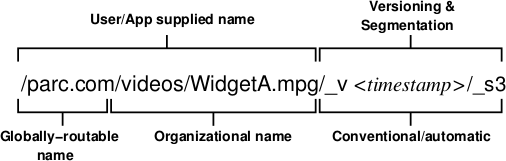
\includegraphics[width=\columnwidth/2]{Images/ndn_name.png}
\caption{NDN name schema example.}
\label{fig:ndn_name}
\end{figure}

Two distinct packets are used to drive communication; interest and data packets. In order to query for data names in the \gls{ndn}, the interest packet is used by the consumer. When this interest packet is received by a node in the \gls{ndn} that has the data (producer), a data packet is returned. This data packets is send back over the same route as the interest packet was sent, resulting in symmetric forwarding. As discussed earlier, data may be cached on the intermediary hops in the \gls{ndn}.

NDN has an advantages over IP, it is able to use multiple paths and unlike IP it is able to handle loops at the forwarding layer. A loop-free topology is realized by inserting a nonce in every interest packet which allows to identify duplicate interests for named data, allowing multiple paths to be used which could increase throughput efficiency. Information about paths in the network are maintained in a layer called the strategy layer. This layer keeps track of two-way traffic and changes local forwarding decisions based on traffic observations. The term 'face' is used in \gls{ndn} to describe a connection to a forwarder, which may be of any class of the underlay (e.g. IP, Bluetooth or any other supported underlay).

The \gls{ndn} packet forwarding engine is composed out of three data structures; The \gls{fib}, \gls{cs} and \gls{pit}. The \gls{fib} is used to forward interest packets towards potential source(s) of matching data. The \gls{fib} allows a list of outgoing faces towards a single prefix. In contrast to an IP FIB, a list for a single destination is not allowed due to network loop problems. The behavior of the forwarding can be changed by using different forwarding strategies. Before an interest packet is send out to the \gls{fib} it is first stored in the \gls{pit} along with the requesting face. An interest packet will remain in the \gls{pit} until a user defined timeout is reached, or when a matching data packet has returned from a source. The prefix and requesting face in the \gls{pit} define a return path back to the requester at each hop, this is referred to as the breadcrumbs path. The \gls{cs} acts as the cache in \gls{ndn}, which is used to provide the distributed property in \gls{ndn}. This cache also has strategies, one for evicting data objects from the cache and one for stashing data objects in the cache.

\subsubsection{NDN strategies}
As described in section \ref{overview-ndn} there are two kinds of caching strategies; a caching decision and a cache replacement strategy. A caching decision strategy is used to determine in which router along the reverse path of an interest packet will cache the data \cite{koulouzis2018information}. The following caching decision strategies are the most well-known.

\begin{itemize}
    \item Leave copy everywhere; used to cache data object packets along each hop in the \gls{ndn} path.
    \item Leave copy down; used only by the first router in the \gls{ndn} path after either the original producer or an \gls{ndn} cache.
    \item Leaving copies with probability; used to cache data objects with the probability of 1/(hop count).
    \item Leaving copies with uniform probability; used to cache data objects with uniform probability.
\end{itemize}

A cache replacement strategy is used to determine which data objects to evict from the cache in order to make room for new data objects. The following cache eviction strategies are the most well-known.
\begin{itemize}
    \item First in first out; used to evict the first data object that was inserted from the cache.
    \item Random replacement; used to evict random data objects from the cache.
    \item Least recently used; used to evict the least recently used data object from the cache.
    \item Least frequently used; used to evict the least frequently used data object from the cache.
\end{itemize}

The information stored in the \gls{pit} and \gls{fib} can be used to determine how to forward an interest packet out to one or more faces. These strategies are meant to give adaptive decisions based on network conditions. The following forward strategies are the most well-known.
\begin{itemize}
    \item Flooding; used to forward received interest packets towards every face, excluding the face the interest originated from.
    \item Best-route with caching; used to calculate the best path with Dijkstra's algorithm (least amount of hops) to reach a data object cache.
    \item Best-route without caching; used to only satisfy interest packets towards the original data publishers, thus excluding intermediary caches along the \gls{ndn} path.
\end{itemize}

\subsection{McCabe}
\label{overview-mccabe}
As briefly described in section \ref{introduction-related-work}, McCabe's book "Network Analysis, Architecture, and Design" \cite{mccabe2010network} is about applying a systems methodology approach towards network design. McCabe's approach consists out of three core phases; analysis, architecture and design. These phases in McCabe describe how to make technology and topology decisions in a network. These decisions are guided based on inputs for these three core phases, the initial input may be from users and/or from network metrics. Consecutive processes use the output of previous processes as input, thus these processes are interconnected. In this section we will describe McCabe's method in more detail.

\begin{figure}[H]
\centering
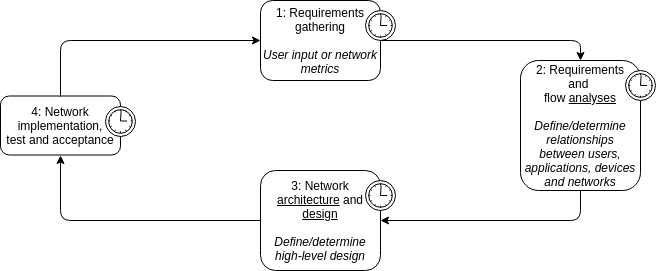
\includegraphics[width=\columnwidth]{Images/mccabe-process.png}
\caption{Cyclic and iterative nature of McCabe's processes and phases.}
\label{fig:mccabe-process}
\end{figure}

In figure \ref{fig:mccabe-process} the three core phases are illustrated in \textit{italic} while the processes are in normal text. In order to highlight the core phases by name they are \underline{underlined} in the figure. The first phase (analysis) has as goal to understand the network and potential problems in terms of performance and efficiency in order to determine network requirements. This is done by developing sets of problem statements and objectives that describe what the target network should address. Therefore, historical data from network management (monitoring), requirements gathered from the network users, staff and management are included in the analysis phase. Furthermore, these metrics are then compared to the relationships between users, applications, devices and other networks in order to determine if requirements match with the user and network expectations. The second and third phase (architecture and design) uses the output of the first phase to establish a high-level design of the network. This network design determines which technology and topology choices are justified to improve the network requirements established in the first phase. The fourth process is implementing the design, test if requirements are met and finally accept the implementation. These phases are intended to be iterative and by no means define a final architecture design. This is due to the fact that requirements, technology and user behavior can change and with that the network design.

\subsection{TOSCA}
\label{overview-tosca}
% Make sure you talk about templates, not just descriptions
% Describe DRIP, OpenStack and an orchestrator in general
\gls{oasis}, an organization which is a global nonprofit consortium that works on open-standards, published the first \gls{tosca} standard in 2014. The \gls{tosca} standard is meant to standardize data modeling for cloud orchestration environments and applications. The latest version 1.1 \cite{tosca-standard}, was released in 2018. In this section we will highlight the important features of TOSCA, relevant to our research scope. Section \ref{planning-deploying} will merge \gls{tosca} with McCabe's method (section \ref{overview-mccabe}).

Portability and automated management of enterprise IT infrastructures are major concerns. Infrastructures may need to run on heterogeneous (cloud) components due to application needs. Having different descriptions of deployment and management for each environment complicates a cloud infrastructure. This challenge introduces new requirements and concepts for deployment, configuration, operation and termination of components that make up an entire infrastructure.

TOSCA provides a single description for a cloud infrastructure consisting out of templates, which is then implemented by an orchestrator. \gls{tosca} orchestrators are e.g. \gls{drip} and OpenStack. \gls{drip} is currently a prototype which uses the open cloud computing interface and currently supports EC2 \cite{amazon-website}, \gls{egi} FedCloud \cite{egi-website} and \gls{exogeni} \cite{exogeni-website} clouds. Furthermore, \gls{drip} also supports Ansible playbooks \cite{ansible-website} for configuration management and contains a deployment agent for e.g. Kubernetes (discussed in section \ref{overview-virtualization}). This results into a portable (can be run by any orchestrator that understands TOSCA) and automated (implementation carried out by an orchestrator) method of infrastructure management. This allows interoperability and reusability of \gls{tosca} template descriptions on different cloud providers. Reusability of templates is made possible by using variables to substitute e.g. IPs or hostnames. These variables can be retrieved with the 'get\_attribute' function and can be declared by a reference node or relationship template \cite{tosca-attributes}.

TOSCA template descriptions consist out of the following core components; nodes, relationships and interfaces. Nodes can be a host, container or VM and are connected to each other through relationships such as 'dependsOn', 'hostedOn' and 'connectsTo'. These relationships can be used to describe that a VM is 'hosted on' a host (e.g. a bare metal machine). Or that a set of containers 'depend on' each other for functionality and 'connect to' e.g. a database. Such as a containerized web application that requires a database, facilitated by another container. Interfaces are used to control the life cycle of a component and consist as a set of hooks to trigger actions, these actions are create, configure, start, stop or delete. These hooks can be triggered to e.g. configure and create containers, stop or start a service or do system maintenance such as delete artifacts after a service is stopped. Furthermore, constraints can be set for the input values in these template descriptions. These can be e.g. that the amount of CPU's should be defined with integers and should contain a value more than one. However, the orchestrator is responsible for verifying these constraints, \gls{tosca} is merely a means to describe components in an infrastructure.

\subsection{Virtualization}
\label{overview-virtualization}
Virtualization provides more efficient use of resources and flexibility because multiple VMs and containers can be deployed on any host that supports them. VMs are virtual operating systems that run in complete isolation from its host. Containers on the other hand share the kernel of its host and offer user-space isolation, which is relatively less isolation when compared to a VM. However, containers are more resource friendly than VMs in terms of needed compute power, memory and disk space. This section will briefly describe these two forms of virtualization. Section \ref{planning-ndn} further applies these virtualization techniques.

Cloud providers such as Amazon provide easy access to compute resources, one way to access these resources is by deploying a VM on their platform. VMs and its resources can be added or removed via management interfaces or APIs. This allows an infrastructure, that e.g. runs on the Amazon cloud platform, to flexibly scale in or out.

Containers offer the ability to package software components together with all dependencies (e.g. libraries and binaries), such a package is called a container image. Docker is a popular platform to build and manage container-based virtualization. Once a Docker image is built it can be distributed through so-called Docker registries, such as Docker Hub \cite{dockerhub-website}. An important property of containers is that they are not persistent, this means that containers revert back to their original image state and that data created inside the container is lost when the container has stopped or crashed. In order to make containers persistent, a data volume can be mapped onto the container's host, thus storing data outside the container.

Kubernetes \cite{kubernetes-website} can be used to automate container deployment, scaling, and management of containers. In Kubernetes a container is called a pod, this may be a Docker container. These Kubernetes pods can be deployed in a cluster of Kubernetes nodes, spanning over e.g. different data centers. This offers great flexibility by packaging an application in a pod and then scale the application in or out through different data centers with Kubernetes. Kubernetes also offers high-availability features, such as automatically restart a pod when a crash occurs or load-balance requests by using a pool of identical pods in e.g. a round-robin fashion. This can be done by configuring a logical set of pods as a service. In order to custom tailor pods, environment variables can be used. These environment variables are then available inside the pod's namespace. Scripts that are executed inside the pod can then use these environment variables to setup e.g. a network configuration by specifying routes and a gateway. In Docker these scripts can be executed via a so called \texttt{ENTRYPOINT} \cite{dockerfile-reference}.

\gls{nfv} is a network architecture concept which uses virtualization to create and manage higher level network functions, as software, on commodity hardware. These functions may be interconnected to create a network service such as load-balancers, firewalls or intrusion detection. This architecture differs from traditional network architectures, where network functions are provided by hardware devices. \gls{nfv} provides the ability to easily duplicate network functionality and expand the network locally or into other data centers. \gls{nfv} is usually managed by an orchestrator to automate deployment, thus providing less overhead than traditional network management with hardware devices.